\documentclass[12pt,letterpaper]{article}

\usepackage{amsmath, amsthm}
\usepackage{graphicx}
\usepackage{microtype, parskip}
\usepackage{caption, subcaption, multirow, morefloats, rotating, longtable}
\usepackage{hyperref}
\usepackage[numbers,sort&compress]{natbib}
\usepackage{authblk, attrib, fullpage}
\usepackage{lineno}


\begin{document}
\begin{titlepage}
  \begin{center}
    \huge{Evolutionary paleoecology and the biology of extinction}

    \vspace{1.5cm}

    \large{Peter D. Smits \\}
    \footnotesize{\href{mailto:psmits@uchicago.edu}{psmits@uchicago.edu}}

    \vspace{1.5cm}

    Dissertation Proposal Hearing \\
    \today \\
    Committee on Evolutionary Biology \\
    The University of Chicago

    \vspace{1.5cm}

    \textit{Committee} \\
    Dr. Michael J. Foote (co-advisor) \\
    Dr. Kenneth D. Angielczyk (co-advisor) \\
    Dr. Richard H. Ree \\
    Dr. P. David Polly
  \end{center}
\end{titlepage}

\tableofcontents
\clearpage

\linenumbers
\modulolinenumbers[2]

\section{Introduction} \label{sec:intro}
%Paleobiology is the study of life over time and the inference of what processes generate the observed patterns in diversity and disparity. Intimately related to paleobiology is the concept of macroevolution here defined as the pattern of speciation and extinction over time \citep{Jablonski2008a}. The study of macroevolution is the estimation of the processes underlying these observed patterns. The term origination is frequently used in place of speciation because it includes both speciation and migration and depending on both the spatial scale and quality of the fossil record it may be impossible to distinguish between the two.
%
Evolutionary paleoecology is the study of the effects of ecological traits and factors on differential rate dynamics, particularly rates of faunal turnover and diversification \citep{Kitchell1985a}. Ecological traits are expressed by a taxon, at any level, and are involved in biotic--biotic or biotic--abiotic interactions while ecological factors are the environmental conditions in which a taxon exists (the set of all biotic and abiotic interactors). Diversification is the difference between origination and extinction and is the net pattern of macroevolution. The study of evolutionary paleoecology is therefore the link between environmental (biotic--biotic and biotic--abiotic) interactions and macroevolution. As a corollary to \citet{Kitchell1985a}'s definition, \citet{Allmon1994} states that in order to correctly link ecological interactions to macroevolution, one must focus on the specific traits and factors that may affect the speciation process. Tacitly included in this is the study of how ecological traits are related to extinction \citep{Kitchell1990}.

It is expectated that for the majority of geological time, extinction is non-random with respect to biology \citep{Jablonski1986} Determining how different traits, both alone or in concert, influence to extinction risk is then extremely important for understanding the differential diversification of taxa over the Phanerozoic. Periods of background extinction also represent the majority of geologic time, remain relatively predictable and change slowly, thus providing a better opportunity to study how traits are related to survival than periods of mass extinction \citep{Jablonski1986,Raup1988}. The Law of Constant extinction \citep{VanValen1973} posits that extinction risk of taxa within a given adaptive zone is age independent (memoryless), however the generality of this statement is possibly suspect \citep{Drake2014,Raup1975,Sepkoski1975,Finnegan2008}. By analyzing the survival patterns within different adaptive zones during periods of background extinction, it should be possible to determine if extinction is best modeled as age independent or dependent.

Organismal traits relating to environmental preference are good candidates for estimating differences in extinction risk. Organismal traits have been shown to be related to differential extinction \citep{Foote2013,Liow2007b,Baumiller1993,Nurnberg2013a}, especially the relationship between adaptation to variable environments and increased species longevity. A simple expectation is that taxa with preference for rare environments will be more at risk than taxa with abundant environments based on purely stochastic grounds. As environments change in availability, a taxon's instantaneous risk of extinction would then be expected change in concert. Taxa are also expected to be adapting to their environment, possibly increasing or decreasing their environmental tolerance and thus changing their instantaneous extinction risk. Related to environmental preference is species-level geographic range size. Species with larger geographic ranges tend to have lower extinction rates than species with smaller geographic ranges \citep{Jablonski1986,Harnik2013,Nurnberg2013a,Jablonski2003,Roy2009c}. However, how range size is ``formed'' is different between clades \citep{Jablonski1987} and thus remains a black box for most taxa. Thus, the utility of focusing on organismal traits related to environmental preference is that the black box can be ``opened.''

% habitat tracking and community connectedness
While the biotic--biotic interactions of a taxon's adaptive zone

It is under this framework that I propose to study how ecological traits associated with environmental preference have affected differential survival and cosmopolitan-endemism dynamics. I will be studying two distantly related and biotically different groups: Permian brachiopods and Cenozoic mammals. Both of these groups are considered to have very good fossil records able to reflect massive long term evolutionary patterns \citep{Mark1977}. These two time periods were chosen because they represent periods of approximately the same length (47 My and 65 My) and of climatic change, global warming and global cooling respectively. Also, these two groups are a marine and terrestrial system respectively and the traits associated with environmental preference and range size (described below) are fundamentally very different. 


Both patterns of survival (Section \ref{sec:surv}) and community connectedness (Section \ref{sec:bionet}) will be measured for both of these groups. The differences between these two groups in terms of life-habit and environmental preference 

% this needs to be improved
Importantly, this comparison allows for a series of questions to be asked with regards to emergent properties and the Law of Constant extinction. Brachiopod and mammal survival can be analyzed at the generic level for different adaptive zones (combinations of traits). The age independence or dependence of extinction for these two groups can then be tested. However because there is a known potential bias towards age-dependent extinction when analyzing generic level survival curves \citep{Simpson2006,Raup1978,Raup1991a}, the mammalian survival will be further analyzed at the specific level and the differences between the two survival functions will be examined, specifically in whether different traits best model the two curves and if either is age-independent or not. Additionally, the importance of global climatic change in modeling both brachiopod and  mammalian survival will be analyzed. In the case of mammalian survival, if global climatic change is found to not be important this does not mean that regional or local climatic changes are not important to survival. By analyzing mammalian community connectedness, it should be possible to estimate how disjoint communities are and if it is reasonable to expect global, regional, or local processes to have dominated and how this may have changed over time.

\subsection{Survival analysis} \label{sec:surv}
Survival analysis is the analysis of time till event data. In the case of paleontological analysis this is the time from the origination (first appearance date; FAD) of a taxon till the time of extinction (last appearance date; LAD), or the duration of a taxon. Survival analysis has a long history in paleontology \citep{Simpson1944,VanValen1973}, though these initial analyses differ from many of the modern approaches \citep{Kleinbaum2005}. Survival is described primarily by two functions, \(S(t)\) and \(h(t)\), or probability of survival at time (age) \(t\) and instantaneous failure rate at time \(t\). The survival function, and corresponding hazard function, can be parameterized in a variety of different ways. 

Survival analysis shares some similarities with linear and logistic regression. While these approaches use continuous (duration) or dichotomous (extinct/not extinct) responses, respectively, survival analysis combines these concepts by measuring the duration till event or follow-up time. In addition to using both duration and death/extinction information, censoring information can also be incorporated in analysis. Censoring is the term for when there is uncertainty of exact survival time and can come in three general forms: right-censored (unknown extinction time), left-censored (unknown origination time), and interval censored (range of possible extinction times). In the case of paleontological survival analysis, censoring provides a framework for the inclusion of taxa ranging into/out of the time period of interest.

The Law of Constant extinction \citep{VanValen1973} predicts that extinction risk is random with respect to taxon age. In the language of survival analysis, this means that \(h(t) = \lambda\) where \(\lambda\) is a constant. This only occurs when survival times are exponentially distributed, formulated as 
\begin{equation}
  S(t) = \exp ^{- \lambda t}
  \label{eq:expsurv}
\end{equation}. Importantly, this observation underlies the ``validity'' of birth-death models of population and clade dynamics where death risk is memoryless.

There are many alternatives to constant extinction risk, however. For example, there is a frequently observed inverse relationship between genus age and extinction risk \citep{Finnegan2008} OTHERS, which could be modeled using, among many others, a Weibull distribution. In comparison to the exponential distribution which has only a single parameter \(\lambda\), the Weibull distribution has two parameters, \(\lambda\) and \(k\). The \(\lambda\) of the Weibull distribution behaves as in the exponential distribution while \(k\) is a shape parameter which describes how failure is proportional to a power of time. If \(k < 1\) then failure rate monotonically decreases with age, and if \(k > 1\) then failure rate monotonically increases with age. When \(k = 1\) the Weibull distribution reduces to the exponential distribution and failure rate is constant. Other potential survival distributions, such as the log-logistic, extended Gamma, and log-normal distributions \citep{Kleinbaum2005}, describe different patterns of age-dependent failure/extinction (monotonic and nonmonotonic).


\subsection{Biogeographic networks} \label{sec:bionet}
Community connectedness is the degree to which localities are composed of endemic versus cosmopolitan taxa, and how similar this ratio is across localities. If localities and taxa are defined as nodes in a bipartite graph, different network measures can be used to measure the how nodes are linked. This then measures both how taxa are distributed among and between localities and how similar different localities are. A bipartite network is defined as a network where nodes can be divided into two disjoint sets such that connections are only between sets and not within sets CITATION, in this case meaning that taxa can only be linked to localities but not to taxa and \textit{vice versa}.

Modified from \citet{Sidor2013}, community connectedness can be measured via four different summary statistics: average relative number of endemic taxa per locality (\(E\), Eq. \ref{eq:e}), average relative locality occupancy per taxon (\(Occ\), Eq. \ref{eq:occ}), biogeographic connectedness (\(BC\), Eq. \ref{eq:bc}), and code length \citep{Rosvall2008,Rosvall2009a,Sidor2013}. These summary statistics describe how unique each locality is on average compared to all others during a time period, how relatively widespread taxa are on average during a time period, how evenly distributed taxa are amongst localities during a time period, and the degree of biogeographic provincially during a time period. Of course, the first three of these measures can be represented as distributions instead of means allowing for better understanding of the spread of taxa over the landscape. 
Three measures are easily defined mathematically. \(E\) is defined as 
\begin{equation}
  E = \frac{\sum_{i = 1}^{L} \frac{u_{i}}{n_{i}}}{L}
  \label{eq:e}
\end{equation}
where \(L\) is as the number of localities, \(u\) is the number of taxa unique to a locality, and \(n\) is the number of taxa present at a locality. This is a measure of how unique localities are on average. \(Occ\) is the number of localities a taxon is, on average, found at and is defined
\begin{equation}
  Occ = \frac{\sum_{i = 1}^{N} \frac{l_{i}}{L}}{N}
  \label{eq:occ}
\end{equation}
where \(N\) is as the number of taxa present in the biogeographic network and \(l\) is the number of localities a taxon occurred in. \(BC\) is a measurement of the shared taxa between localities and is defined 
\begin{equation}
  BC = \frac{O - N}{LN - N}
  \label{eq:bc}
\end{equation}
where \(O\) is the total number of taxonomic occurrences. \(BC\) ranges from 0 to 1, with 0 meaning that each locality completely disconnected from all other localities and 1 indicating that all taxa are presents at all localities. 

Code length is a measure of the information flow \citep{Shannon1948} of a graph as estimated from the behavior of a random surfer \citep{Brin1998} on a graph and how often it visits each node and it's behavior with regards to moving into and out of different regions of the graph. Code length is the minimum length of a binary code for describing the behavior the surfer and the community structure of the nodes and is estimated via the map equation \citep{Rosvall2008,Rosvall2009a}. The logic of the map equation is that a good map compresses reality into as few symbols as possible thus we want to compress as many nodes as possible into as few symbols as possible. Our goal is to represent a graph better than just assigning a unique Huffman code to each node \citep{Huffman1952,Rosvall2008}. By compressing multiple nodes into a single code block, we decrease the minimum coding length of a network and a network with a low code length has more nodes compressed into distinct subunits/provinces without losing the underlying information flow of the graph. In the case of measuring community connectedness, a low code length means greater site distinctness and provinciality than a graph with a high code length \citep{Sidor2013}. For further examples of the map equation, visit \url{http://mapequation.org/}.

Analysis of these measures of community connectedness both within and between different regions across the globe allows for the expected relative importance of global versus regional versus local scale processes, and how this might change over time, to be estimated. If global processes are important to patterns of community connectedness and environmental interactions than it is expected that these measures will be correlated with global climate measures. Additionally, if two or more regions have similar or correlated patterns of community connectedness, it is expected that global processes may play a roll in shaping the environment. Regional processes are expected to dominate when \(E\) is low, \(Occ\) is high, \(BC\) is high, and code length is high. In contrast, local processes are expected to dominate when \(E\) is high, \(Occ\) is low, \(BC\) is low and code length is low. The different scales are not mutually exclusive, however, and one or more scales might be involved in shaping patterns of community connectedness and environmental interactions. Importantly, which process scales are dominant may change over time.


\section{Australian Permian Brachiopods} \label{sec:brac}

\subsection{Traits and environmental preference} \label{sec:bracback}
Brachiopods are suspension feeders that are not actively motile, thus the availability of optimal environmental conditions is extremely important for both establishment and survival. Brachiopod occurrence has been found to be strongly linked to the type ocean floor on which they occur \citep{Richardson1997,Richardson1997a}. Environmental preference is esteemed here using three traits, two environmental and one biological: substrate preference, habitat preference, and surface interface/affixing strategy. Each of these three traits relates to a different aspect of the environment and a taxon's specific adaptive zone. Importantly, it is possible that the loss of suitable environments may determine different trait associated extinction risk. While larval mode is considered an important trait associated with geographic range and extinction risk \citep{Jablonski2006a,Jablonski1983}, it does not perserve in brachiopods and thus cannot be used to model survival \citep{Jablonski1983}. Additionally, taxa found on the east coast of Australia during the Permian would have been facing the Panthalassic Ocean and would have had few ``good'' areas to disperse to except in the immediate region because of the distance required to reach a different shore line and the high latitude of the region.

Substrate preference is related to the chemical and physical processes affecting a given environment. Substrate selection is mitigated via larval chemosensory abilities and thus may act as a weak proxy for larval dispersal ability \citep{Jablonski2006a,Jablonski1983}. The three generally used states of substrate affinity are carbonate, clastic, or mixed \citep{Foote2006,Anderson2011a,Nurnberg2013a,Kiessling2007a,Miller2001}. The Pharenozoic is characterized by an overall decline in carbonates relative to clastics \citep{Foote2006,Miller2001}. Additionally, the Australian Permian is dominated by clastic beds \citep{Birgenheier2010,Percival2012,Thomas2007,Fielding2008a,Fielding2008}. It is expected then that the majority of brachiopod taxa will prefer clastic type substrates compared to the rarer carbonate type substrates.

Habitat preference is a description of the depositional environment in which a taxon was found at the time of fossilization. Because brachiopods are sessil and frequently fixed to the environment, it is expected that the inferred depositional environment is akin to that in which they lived. The range of depositional environments are quite broad, representing many different marine settings. Because of the large range and difficulty of precisely inferring depositional environment a frequently used, albeit coarse, classification is on-shore versus off-shore \citep{Sepkoski1991,Kiessling2007a,Bottjer1988,Jablonski1991,Jablonski1983b} along with the option of a taxon having no particular habitat preference. Importantly, habitat availability is broadly related to sea-level which can change both dramatically and rapidly over time \citep{Olszewski2004}. Because of this, on-shore type habitats are potentially very volatile and unstable for long periods of time. During the Permian of Australia there were four major glaciation events which covered most of the entire continent \citep{Fielding2008,Birgenheier2010,Fielding2008a,Fielding2006}, which most likely strongly impacted sea-level as well as the availability and constancy of on-shore versus off-shore habitats. Additionally, habitat might capture other factors relating to the environment not captured in substrate preference. 

Affixing strategy is the manner by with an individual interfaces with the environment. Unlike bivalves which can burrow or snails which are motile, a brachiopod is sessil and has to maintain their commisure at or above substrate level in order to expose their lophophore. Because of this, brachiopods have evolved a variety of different methods to position themselves in various different environmental conditions such as flow speed or mud depth \citep{Alexander1977,LaBarbera1978,LaBarbera1981,Richardson1997}. Broadly, these methods can be classified as pedunculate (presence of a pedicle), reclining (absence of pedicle), and cementing. During the Permian, pedunculate taxa are associated with shallow on-shore environments while reclining taxa are associated with deep off-shore environments \citep{Clapham2007} however these associations are weak as most assemblages are composed of a heterogeneous mix of strategies.

Additionally, the Permian shift from an ``ice house'' to a ``hot house'' world \citep{Fielding2006,Birgenheier2010,Jones2006,Powell2007,Fielding2008}. Australasian taxa are of particular interest because of their proximity to the south pole during the Permian and the repeated glacial activity in the region \citep{Fielding2008a,Fielding2006,Birgenheier2010,Jones2006}. According to \citet{Olszewski2004}, however, sea-level and climate change do not wholly explain the brachiopod ecological dynamics experienced in the Permian of Texas. It is then predicted that climate will not be the best sole predictor of brachiopod survival, and that some combination of one or more the above organismal traits will be necessary to best model survival. 


\subsection{Environmental preference and extinction} \label{sec:bracsurv}
\subsubsection{Questions} \label{sec:bracsurvques}
Which traits relating to environmental preference in brachiopods are predictors, either separate or together, of differential survival? Do Permian glacial periods relate to differences in trait-correlated extinction? What is the distribution of brachiopod generic survival?

\subsubsection{Hypotheses and predictions} \label{sec:bracsurvpred}
Because of both the long-term decline in carbonates versus clastics \citep{Peters2008} and the dominance of Permian-age clastic beds \citep{Birgenheier2010,Percival2012,Thomas2007,Fielding2008a,Fielding2008} described above (Section \ref{sec:bracback}), it is taxa with clastic type affinities will have longer durations than taxa with any other preference. Additionally, this substrate dominance may have been a heavy selection pressure for taxa to adapt to common clastic types and/or away of the rarer carbontes.
Because of this, it is expected that taxa with clastic or mixed affinities will have greater survival than taxa associated with carbonate substrates. Additionally, it is predicted that substrate preference, if it captures the same information as modern substrate type, will be a predictor in the best model(s) of survival \citep{Richardson1997,Richardson1997a}. However, if substrate affinity is not found to be important for modeling survival this may be due to one or more reasons. First, substrate affinity, as quantified here, may not be capturing the same information as modern substrate type and thus may act as a poor predictor of survival. Second, it may mean that because clastic type substrate were so dominate during the Permian of Australia that differential survival may be better explained by other factors, either measured or unmeasured. 

While other environmental factors beyond substrate type, such as temperature or water depth, have not been found to limit the distribution of modern brachiopods \citep{Richardson1997,Richardson1997a} it is unknown if these traits affect survival. Predictions of differential survival based on habitat preference and affixing strategy can be made on the basis of environmental preference and availability.

During the Permian of Australia there were four major glaciation events where the most of the continent was covered \citep{Fielding2008,Birgenheier2010,Fielding2008a,Fielding2006}, it is expected that off-shore adapted taxa will have greater durations than on-shore adapted taxa. This prediction is based on the expected constancy and availability of off-shore habitats and the expected high volatility of on-shore habitats. If habitat preference is not found to be a predictor for modeling survival, this may mean that sea-level mediated environmental availability does not determine long term survival. Specifically, while sea-levels may have fluctuated greatly due to high latitude glaciation \citep{Fielding2008,Fielding2008a,Birgenheier2010} it may be that the long term continual availability of habitat over-shadows short term fluctuations. Also, it has been found in the case of Permian brachiopods from Texas that sea-level along with climate change do not wholly explain the observed ecological dynamics \citep{Olszewski2004}, which may mean that habitat availability may not be the singly dominate factor when modeling brachiopod survival. Additionally, in the case that habitat preference is a good predictor of survival but not the ``best'' this may mean that other factors may be more dominate factors related to survival.

Previous global level analysis of brachiopod durations showed that affixing strategy is correlated with longevity \citep{Alexander1977} and that among endemic taxa, reclining taxa had longer durations than other affixing strategies. Among cosmopolitan taxa, however, pedunculate and cementing taxa had longer durations than all other taxa, both cosmopolitan and endemic. This global analysis mixed taxa from many different geological periods and geographic regions which may produce unfair and biased comparisons. By restricting analysis to a single continuous region, I hope to alleviate these concerns and instead focus on survival of an evolving taxonomic assemblage in a continuous environmental context.  If affixing strategy is found to not be a predictor in the best model(s) of survival this would mean that, while it is correlated with differential survival \citep{Alexander1977}, it may only be a minor factor. For example, this may indicate that the environmental energetics of Australasia was rather uniform. 

An important consideration is that taxonomic survival might not be linked to single environments \textit{per se}, but the variability of environments \citep{Foote2013,Heim2011,Liow2007b}. Adaptation to environmental variability has been found to relate strongly with survival past origination \citep{Foote2013}. Adaptation to variability of environments may be captured in taxa with mixed substrate preference and/or no habitat preference. Based on this observation, it is predicted that taxa with mixed substrate preference and/or no habitat preference will have longer durations than taxa with single preferences. However, this may also mean that taxa with mixed substrate and/or no habitat preferences will be of similar duration to clastic type and off-shore preferences, which are predicted to have the longest durations for their respective traits.


\subsubsection{Proposed research} \label{sec:bracsurvmeth}
%ERLANG distribution: sum of \(k\) independent exponential variables with mean \(\mu\)
%HYPOEXPONENTIAL distribution: genearlized ERLANG distribution

In order to investigate which traits best model survival and how, I propose a survival analysis approach as described above (Section \ref{sec:surv}). I choose to restrict this analysis to Australasia because it represents a relatively continually sampled and well worked area that preserves the majority of the entire Permian \citep{Fielding2008,Birgenheier2010,Clapham2012,Clapham2008a,Waterhouse1987,Archbold1995}.

Permian brachiopod occurrence information is available via the Paleobiology Database (PBDB; \url{http://fossilworks.org}) and is primarily based on the work of Clapham \citep{Clapham2006,Clapham2008a,Clapham2007a,Clapham2012,Clapham2007} and \citet{Waterhouse1987}. While lithological and paleoenvironmental information is available for some occurrences through the PBDB, this information is frequently missing or too coarse. Lithological information and paleoenvironmental reconstructions will be heavily supplemented using the extensive geological unit information from Geosciences Australia (\url{http://www.ga.gov.au/}) as well as the literature on the stratigraphy of Australian Permian basins CITATIONS


Because substrate and habitat occurrences are not constant at the species level, it is necessary to determine the most probable assignments. The lithology of all occurrences will be classified into one of the three substrate affinity categories following \citet{Foote2006} while paleoenvironmental setting of all occurrences will be classified into one of the habitat preferences following \citet{Kiessling2007}. Both of these traits will be assigned to all taxa following the Bayesian approach of \citet{Simpson2009} where assignments are determined as the posterior probability of a taxon's occurrences in comparison to available options during the duration of said taxon. Assignment probability, \(P(H_{1}|E)\), will be calculated as
\begin{equation}
  P(H_{1}|E) = \frac{P(E|H_{1})P(H_{1})}{P(E|H_{1})P(H_{1}) + P(E|H_{2})P(H_{2})}
  \label{eq:aff}
\end{equation}
where \(P(H_{1})\) and \(P(H_{2})\) are the prior probabilities of assignment while \(P(E|H_{1})\) and \(P(E|H_{2})\) are conditional, binomial probabilities. 

% table of models w/ linked hypotheses

Multiple models of survival with various combinations, both additive and interactive, of the traits described above will be compared. Substrate preference, affixing strategy, and habitat preference will be assumed to be constant for the duration of the taxon and modeled as time-independent covariates. If and how these traits may have evolved will remain for future study. Climate change will be modeled as either an ancillary Heaviside function or an ancillary time-dependent covariate.



\subsubsection{Preliminary results} \label{sec:bracsurvres}
Preliminary analysis of brachiopod survivorship was restricted to genera that originated within the Permian. Survival was analyzed for taxa classified for substrate affinity and habitat preference. For substrate affinity, the priors of Eq. \ref{eq:aff} were \(P(H_{1}) = P(H_{2}) = 0.5\) and if \(P(H_{1}|E) > \frac{2}{3}\) then the taxon was considered of carbonate affinity while if \(P(H_{1}|E) < \frac{1}{3}\) then the taxon was considered to have a clastic affinity. Otherwise, the taxon was considered to have mixed affinity. In the case of habitat affinity, the posterior probability for each habitat (inshore, offshore, none) was calculated using Eq. \ref{eq:aff} with priors of \(P(H_{1}) = \frac{1}{3}\) and \(P(H_{2}) = \frac{2}{3}\) and the preference with maximum of the three posterior probabilities was the assignment.

Preliminary model fitting with both exponential and Weibull distributions and either or both traits indicated that the best model, based on comparison of AICc scores \citep{Hurvich1989,Akaike1974,Burnham2002a}, was the model with substrate affinity as the sole predictor and a Weibull distribution of survival. This model is illustrated below (Fig. \ref{subfig:aff_surv}). While this is the preliminarily best model of survival, the model with both substrate affinity and habitat preference as additive effects and a Weibull survival distribution may also be considered a good model of survival (\(\Delta\)AICc \(\approx 2.9\)). Additionally, as illustrated by the difference between the nonparametric Kaplan--Meier survival curves and the predictions of the parametric model of survival (Fig. \ref{subfig:aff_surv}) and there is room for improvement in model specification.

\begin{figure}[t]
%  \begin{center}
  \begin{subfigure}[b]{0.5\textwidth}
    \caption{}
    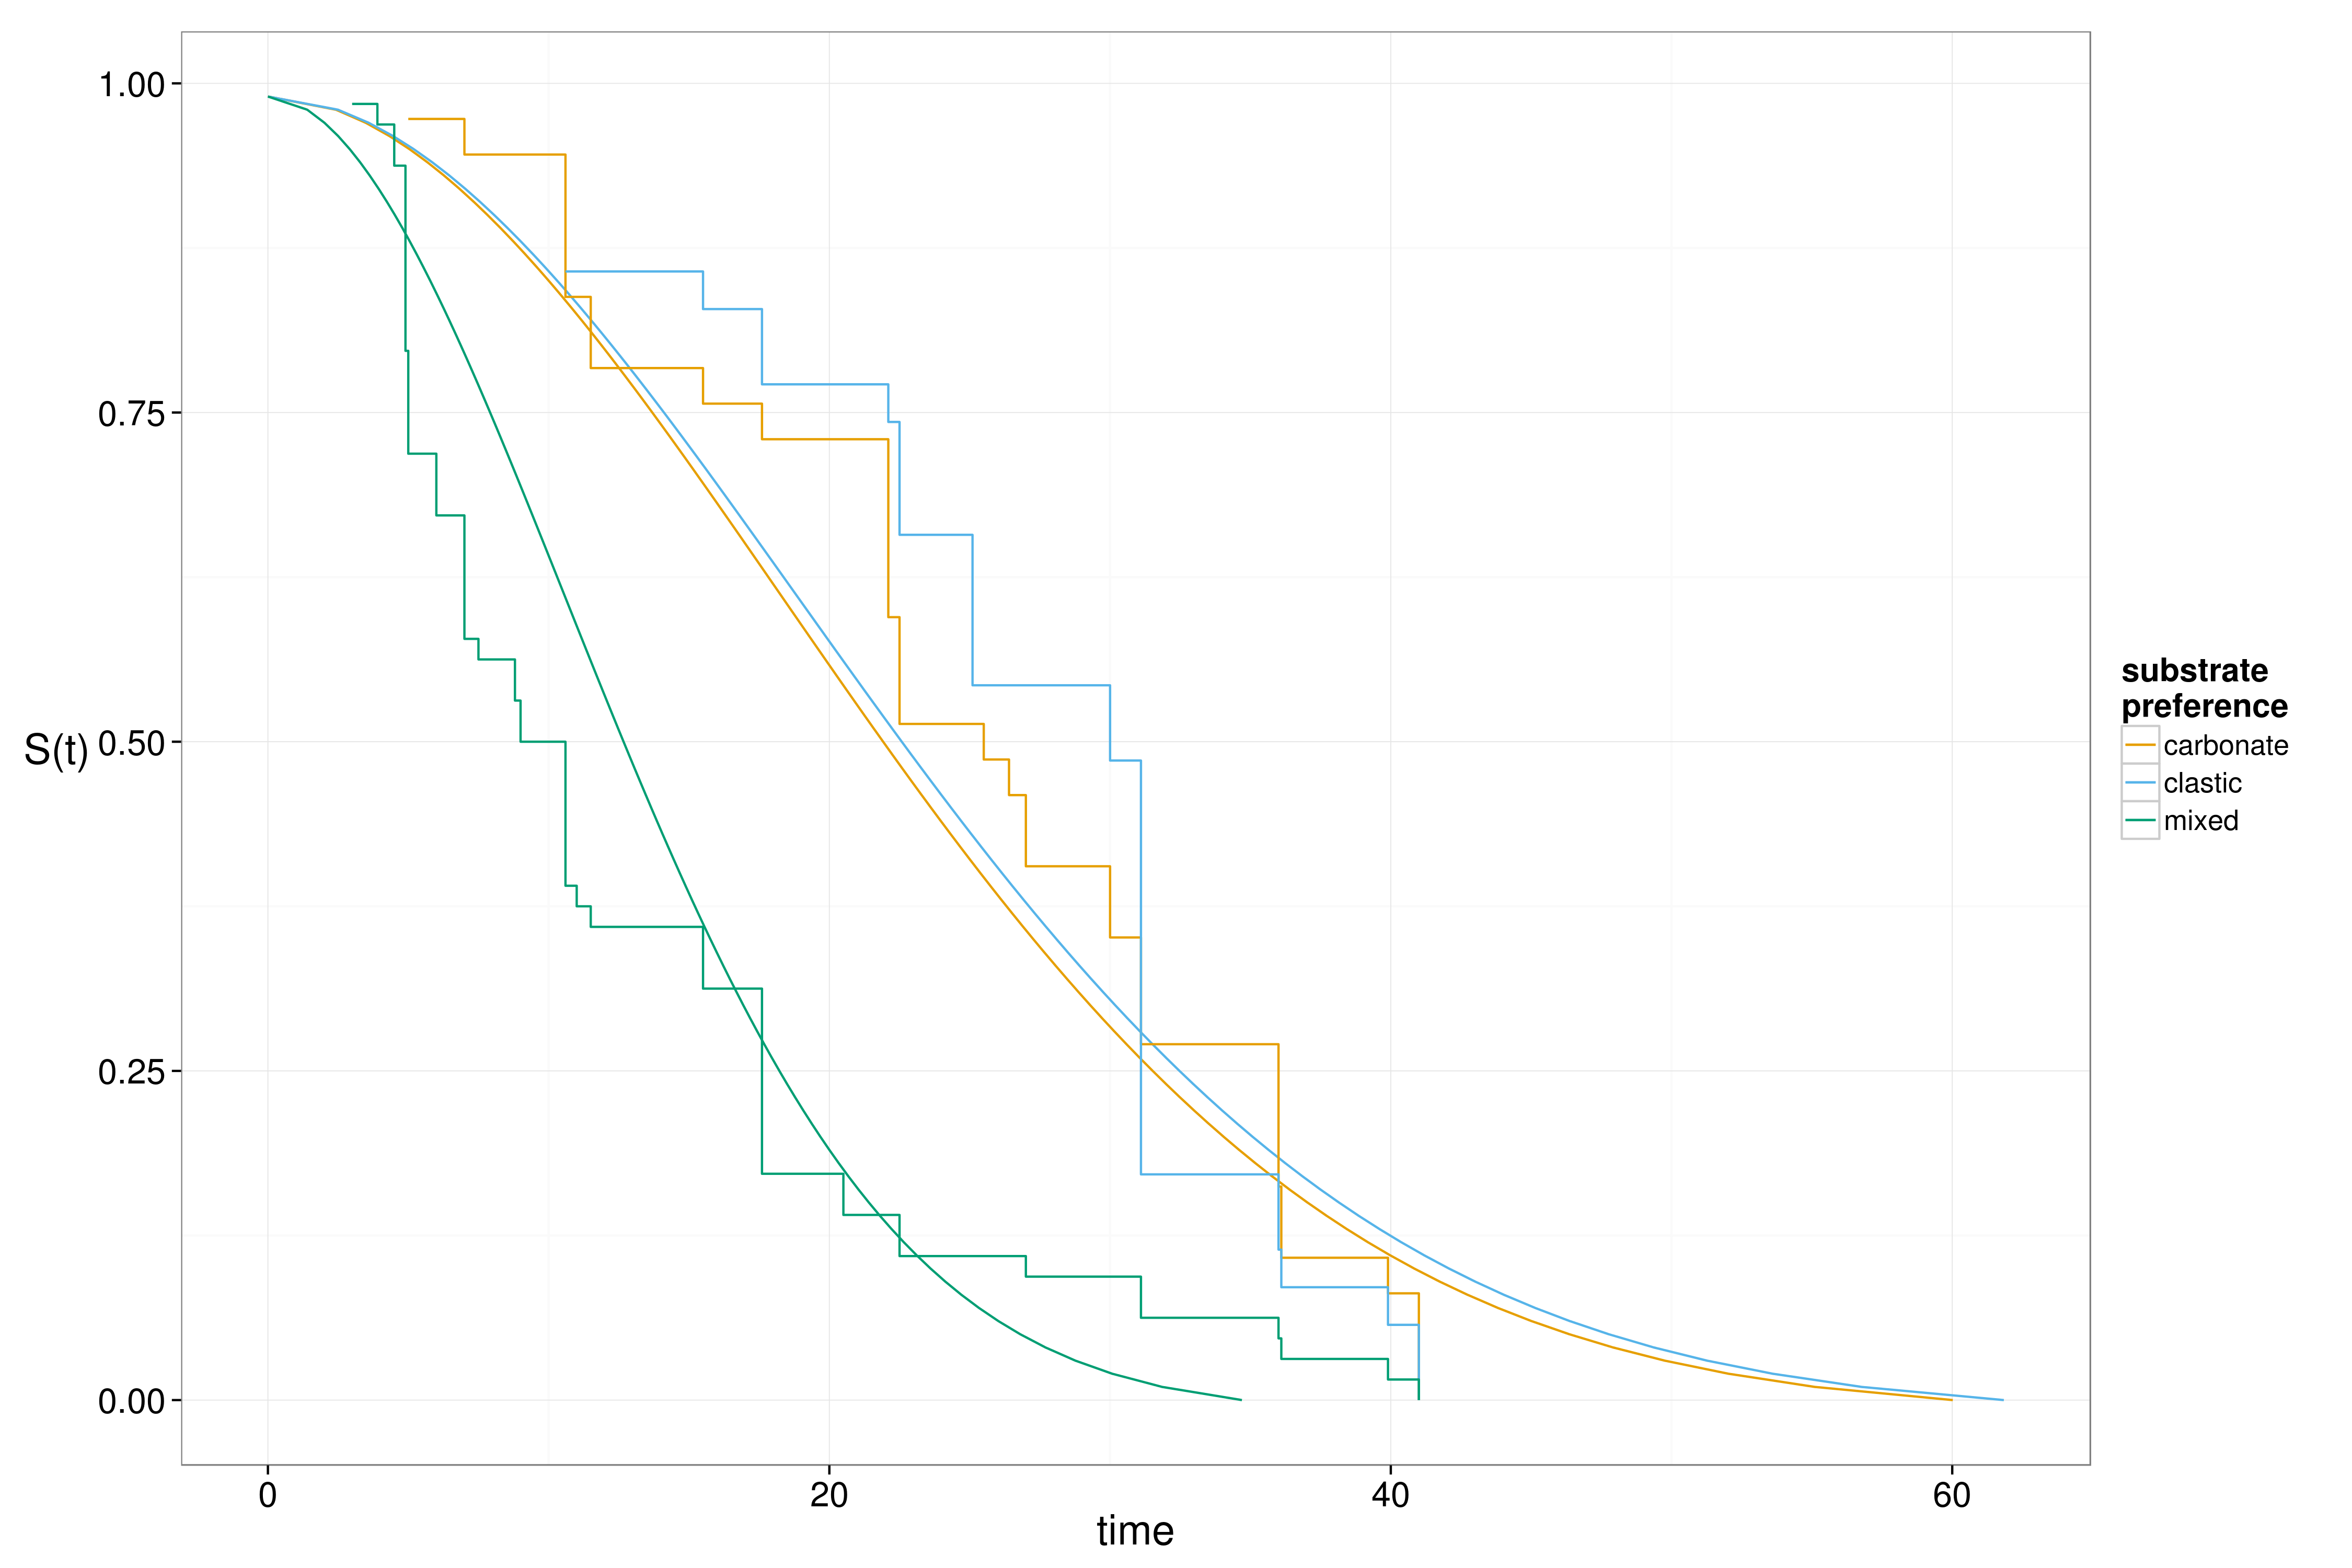
\includegraphics[height = 0.4\textheight, width = \textwidth, keepaspectratio = true]{figure/aff}
    \label{subfig:aff_surv}
  \end{subfigure}
  \begin{subfigure}[b]{0.5\textwidth}
    \caption{}
    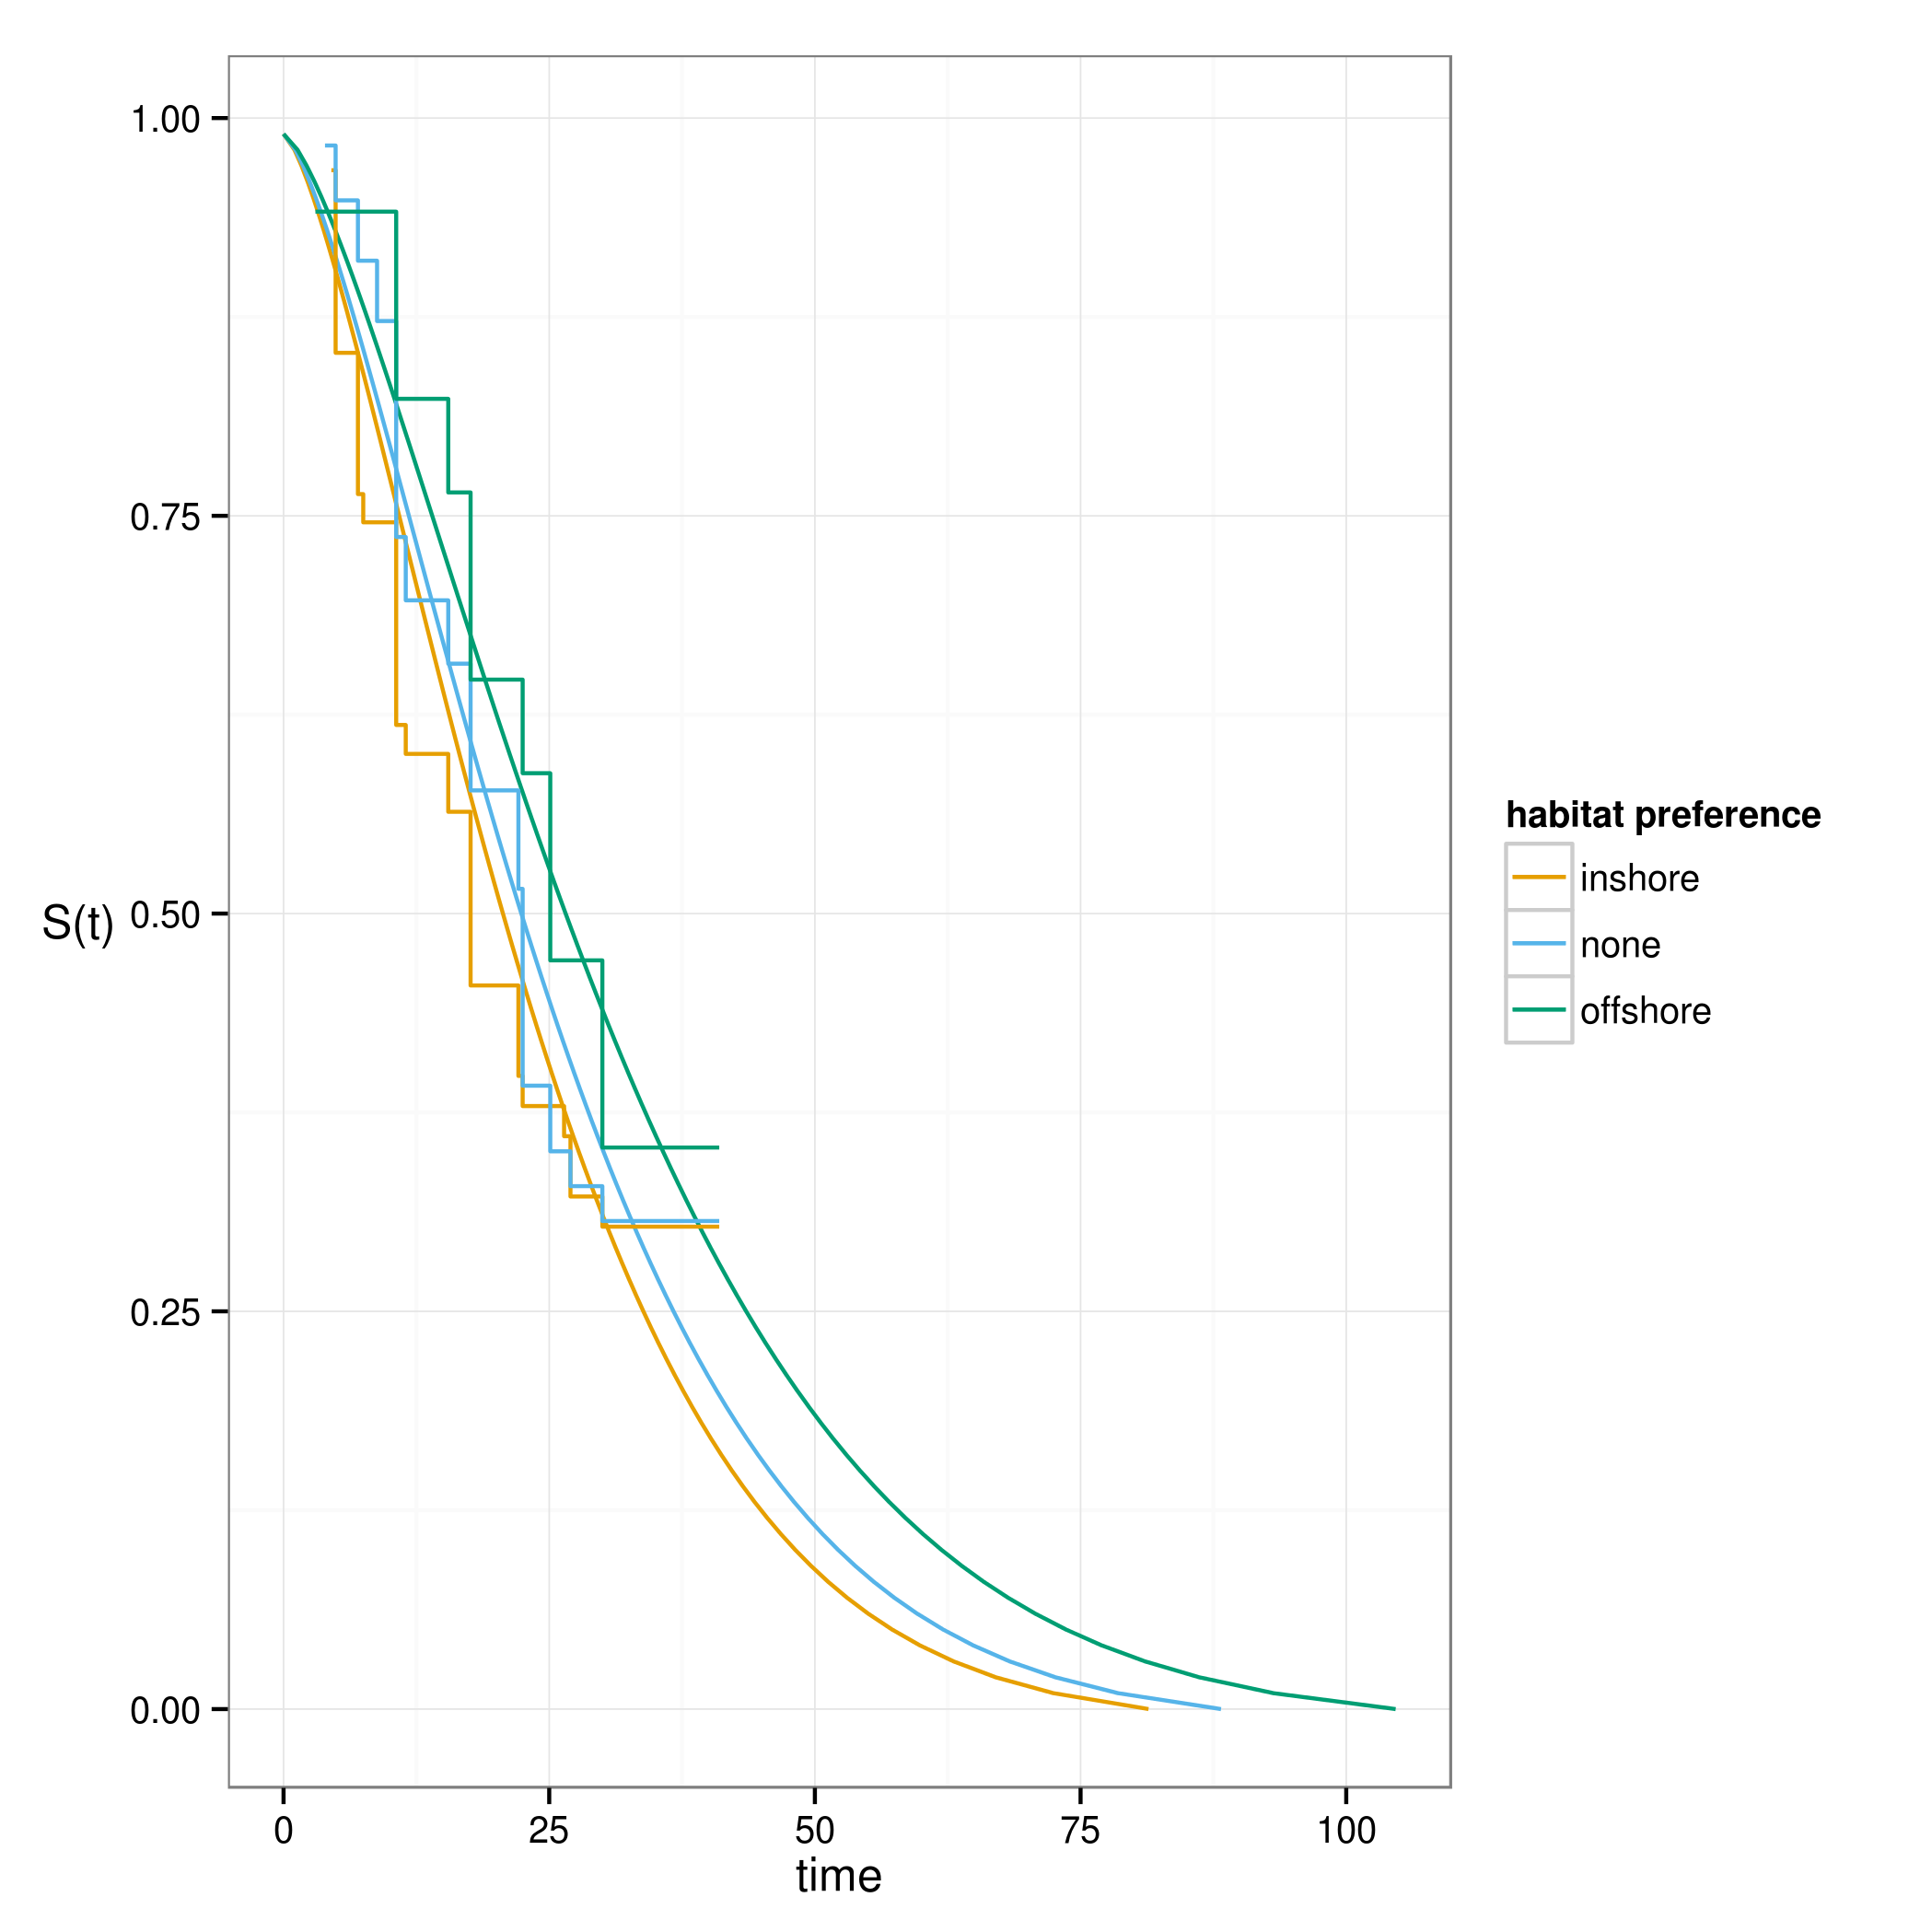
\includegraphics[height = 0.4\textheight, width = \textwidth, keepaspectratio = true]{figure/hab}
    \label{subfig:env_surv}
  \end{subfigure}
%  \end{center}
  \caption{Survivorship curves of Australasian Permian brachiopod genera based on substrate affinity (\subref{subfig:aff_surv}) and habitat preference (\subref{subfig:env_surv}). The stepwise functions are nonparametric Kaplan--Meier survival curves for each of the three substrate affinities. The three smooth lines are the predicted survivorship probabilities for taxon of the given age from parametric survival models.}% and illustrated standard errors of the prediction.}
  \label{fig:brach_surv}
\end{figure}

The shape parameter (\(k\)) of the AICc best model (Fig. \ref{subfig:aff_surv}) is estimated to be approximately 1.9. As described above, values of \(k\) greater than 1 indicate that failure (extinction) rate is accelerating with respect to taxon age, which may mean that the Law of Constant Extinction does not hold when modeling generic level extinction in brachiopods.

For brachiopod survival based on substrate affinity (Fig. \ref{subfig:aff_surv}), survival was greater for both carbonate and clastic affinities and lowest for taxa with mixed affinity. Visual inspection of the estimated survival functions compared to the nonparametric Kaplan--Meier curves indicates that they were adequate fits to the data. 

Brachiopod survival with the sole predictor being environmental and a Weibull distribution of survival was not a good model of survival, with an approximate \(\Delta\)AICc of 33 between this model and the AICc best model. There is a great degree of deviance between the nonparametric Kaplan--Meier curves and model predictions (Fig. \ref{subfig:env_surv}). Additionally, this model is not significantly different from the model with only an intercept (\(\chi^{2} = 2.41\), \(df = 2\), \(p = 0.3\)). This means, preliminarily, that habitat preference alone makes no difference in generic level survival.

Further refinements to these models include modeling survival using other distributions of survival such as a log-normal distribution. Additionally the inclusion of affixing strategy and climate as predictors will increase the understanding of the biology underlying brachiopod generic survival. Additionally, the effects of sampling and uncertain durations will explored in simulations described below in the context of generic versus specific survival.




\section{Ecology and survival in Cenozoic mammals} \label{sec:mamsurv}

\subsection{Questions} \label{sec:mamsurvques}
How do ecological traits related to range size affect mammalian taxon duration? Is any single trait the best predictor of mammalian survivorship, or do multiple traits together best model taxon duration? Is climate an important factor in modeling mammalian taxon duration?

\subsection{Background and Predictions} \label{sec:mamsurvback}
Three potential constituent traits of range size in mammals are dietary category, locomotor category, and body size \citep{Smith2004,Smith2008b,Damuth1981a,Damuth1979,Jernvall2004,Lyons2005,Lyons2010}. These traits describe different aspects of how an organism interacts with the environment based on either prey availability, dispersal ability, or energetic cost. Dietary categories are defined here as broad trophic categories that subsume further, more specific, classifications. The categories used here are carnivore, herbivore, omnivore, and insectivore. It should be noted that most prior analyses have not included insectivore as a category \citep{Jernvall2004,Price2012}. Similarly, locomotor categories are defined as combinations of more specific classifications and are broken into arboreal, ground dwelling, and scansorial. Both of these traits are constant at the specific level. 

Dietary categories limit abundance because of the availability of resources in a location \citep{VanValen1989,Brown1987,Damuth1979,Silva1997,Janis2000}. Abundance is correlated with occupancy, or the number of localities at which a taxon is found \citep{Jernvall2002,Fortelius2002,Brown1984}. It follows then that the limits on abundance imposed by resource availability would affect the possible range size of a taxon. Because dietary categories are fundamentally linked to primary productivity and trophic hierarchy, it is expected that the most stable categories would have the greatest survival and the least stable would have the lowest survival. Stability is used here to mean number of ``steps'' from primary productivity and the related relative requirement of other biotic interactors. As such, herbivores are expected to have greatest survival and carnivores the lowest survival. Omnivorous taxa are expected to have average taxon durations compared to the other two categories. Mammalian herbivores and carnivores have been found to have a greater diversification rate than omnivores \citep{Price2012} which may indicate that these traits are better for survival. However diversification can be caused either by an increase in origination relative to extinction or a decrease in extinction relative to origination. If the latter scenario occurred, this would agree with the predictions from \citet{Price2012} that herbivorous and carnivorous taxa would be more successful and have had greater average survival than omnivores. Which scenario occurred, however, is (currently) impossible to determine from a phylogeny of only extant organisms \citep{Rabosky2010a} which means that analysis of the fossil record is necessary to estimate which scenario was most likely. If dietary category is not found to be important for modeling survival it may mean that trophic category is not a major factor for determining species level survival and that other factors, such as body size, may dominate. 

Locomotor category describes the motility of a taxon and the plausibility of occurrence. For example, an obligate arboreal taxon can only occur in locations with a minimum of tree cover and can most likely only disperse to other environments with suitable tree cover. Dispersal ability is considered important in determining the extent of a taxon's geographic range \citep{Birand2012,Jablonski2006a,Gaston2009} and thus any trait that limits dispersal ability would most likely also limit the range size of that organism and increase extinction risk. During the Cenozoic, between the Paleogene--Neogene, there was a shift from a predominately closed environment to a predominately open environment \citep{Janis1993a,Blois2009,Rose2006}. It is expected then that arboreal taxa during the Paleogene will have a greater expected duration than Neogene taxa, and the opposite will be true for ground dwelling taxa. In comparison, taxon duration of scansorial taxa is expected to remain relatively similar between the two time periods because it represents a mixed environmental preference that may be viable in either closed or open environments. If locomotor category is not included in the best model of survival this may mean that it is either a poor descriptor of potential dispersal ability or range size or that other factors, both measured or unmeasured, may be of greater importance. The difficulty of a Paleogene--Neogene comparison, which is potentially underminded by heterogeneous preservation potential, will be explored in simulation as described below.

Similar to dietary category, body size has an associated energetic cost in order to maintain homeostasis, which in turn necessitates a sufficient supply of prey items. Because of this, it is expected that larger organisms have higher energetic costs and thus a greater range size in order to obtain necessary resources \citep{Damuth1979,Brown1987,Damuth1979,Lyons2010}. It is then expected that, because taxa with larger range sizes have been found to have lower extinction rates, that species with higher average body sizes will have a lower extinction rate than taxa with smaller body sizes. This expectation, however, may not be right. As body size increases, reproductive rate decreases \citep{Johnson2002b}, populations are smaller \citep{White2007}, generations are longer \citep{Martin1993a} all of which can increase extinction risk, as has been observed \citep{Liow2008,Davidson2012}. However, the relationship between body size and extinction rate at the generic level has been found to vary between continents \citep{Tomiya2013,Liow2008}. By expanding to include a third continent, South America, and analyzing specific level data I hope to elucidate how differences in taxonomic diversity at a continental level might affect body size mediated extinction rate. If body size is found to be unimportant for modeling survival, as in the generic level analysis of \citet{Tomiya2013}, this means that other biotic or abiotic factors may dominate. This may also mean that individual level home range size does not scale into increased species level range size, and there is therefore no correlated decrease in extinction rate. 

The interaction of body size, locomotor category, and dietary category is also extremely important. For example, a small bodied arboreal taxon of any trophic category during the heavily forested and warm time of the Paleogene would be expected at once to have both a small body size determined range, a large potential geographic range determined by locomotion, as well as an increased availability of resources. Together this would mean that relative survival would be expected to be less than, greater than, and greater than average respectively. Determining which factors dominate during the Paleogene, as well as other parts of the Cenozoic, must be done empirically.


\subsection{Proposed research} \label{sec:mamsurvmeth}
To analyze differential mammalian survival, I propose a survival analysis approach similar to that described above for Permian brachiopods. Because dietary category and locomotor category are constant at the species level, they will be modeled as time-independent covariates of survival. While a taxon's average body size may evolve over time, the resolution of the mammal fossil record does not permit observation of this for all Cenozoic taxa. Instead, following previous work, body size will be considered constant with respect to time and will also be modeled as time-independent covariate. The climate proxy \(\delta O^{18}\) oxygen curve \citep{Zachos2008} will be modeled as an ancillary time-dependent covariate. Also, as described above for Permian brachiopods, constant versus age dependent extinction rate will be tested by comparing the fit of survival to various probability distributions. Additionally, the effect of stratification based on the Paleogene--Neogene divide will be assessed in order to determine if the time periods had distinct patterns of survival. For this Paleogene--Neogene comparison, the principle interest will be with differences in relative trait--based survival between time periods and not with exact estimates.

While many analyses of survivorship, such as the one described above for Permian brachiopods, are done using generic data \citep{Tomiya2013,Liow2008,Harnik2013}, there are potential biases in accurately modeling specific level processes using generic level data \citep{Raup1975,Sepkoski1975,Simpson2006,Raup1991a,VanValen1979}. In order to assess some of the differences between generic and specific level survival, I will estimate specific and generic level survival models. Using an approach similar to previous work on estimating specific level origination and extinction rates from generic level survival curves \citep{Foote1988}, I will measure the deviance between extinction rate directly estimated from the specific survivorship and the specific level extinction rates estimated from the generic level survival data. In addition to empirical comparison between generic and specific level survival, simulations of diversification with varying levels of cryptic speciation (anagenesis). This may also act as a proxy for generic level diversification because a lineage having a long duration because it is not correctly broken up can be considered analogous to a genus persisting because it continues to speciate.

Homogeneous preservation across taxa is expected to have a minimal and uniform effect on estimates of duration and survival \citep{Sepkoski1975}. However, the above comparison between the Paleogene--Neogene may be biased due to heterogeneous preservation between environments. Differential preservation between open and closed environments might strongly bias taxon duration estimation and strongly bias comparisons of survival. I propose a series of simulations in order to explore the effects of heterogeneous preservation on survival: two groups with identical diversification and identical preservation, two groups with identical diversification but different preservation, two groups with different diversification but identical preservation, and two groups with different diversification and different preservation. Because phylogenies are frequently simulated as a time-homogeneous birth-death process, this will be the model used to simulate diversification. The expected survival distribution for a time-homogeneous birth-death process is exponential because of the age independent rate parameter (\(\lambda\)). 

Mammalian occurrence data will be collected primarily through a combination of the PBDB, Neogene Old World Database (NOW; \url{http://www.helsink.fi/science/now/}), and museum collections. North American fossil mammal data are well represented and vetted in the PBDB because of the extensive work of Alroy \citep{Alroy1996a,Alroy1998,Alroy2000g}. European fossil mammal data is also well represented between the PBDB and NOW. South American fossil mammal data is available through the PBDB, but is not particularly well vetted and has poor overall coverage. Because of this, South American fossil mammal data will be gathered via various museums such as the Field Museum of Natural History and the American Museum of Natural History as well as published occurrence compilations. With the South American taxa, taxonomy and sampling may not be as well resolved as for North and South America and it may be necessary to restrict analysis to the most taxonomically resolved and sampled groups such as Notoungulata, Marsupials, Carnivora, and Primates.


\section{Community connectedness in Cenozoic mammals} \label{sec:mamcom}

\subsection{Questions} \label{sec:mamcomques}
How does community composition change over time in terms of the ratio between endemic and cosmopolitan taxa? Is there a single global pattern, or do different continents have different patterns? Do patterns differ between ecological categories? Is global climate change an important predictor of these patterns?

\subsection{Background and Predictions} \label{sec:mamcomback}
How community composition changes over time and in relation to organismal traits and a changing environment is extremely important for understanding how trophic structure changes or is maintained over time. Additionally, community connectedness is important for understanding the degree to which global, regional, or local scale processes are important for shaping environmental interactions, both biotic--biotic and biotic--abiotic.

In addition to total community connectedness, the dynamics of taxa within various ecological categories are important for understanding whether different adaptive zones may be differently affected by global, regional, or local scale processes. As described above, two important traits for potentially determining range size in mammals which are constant at the specific level are dietary category and locomotor category. 

During the Cenozoic there was a global shift from closed, forested habitat to open, savanna-like habitat. Importantly, the timing of this environmental shift was different between continents \citep{Stromberg2005,Stromberg2013}, so patterns of community connectedness may not be globally uniform and could reflect regional differences. The global prediction is that there would have been a relative increase in \(E\) and code length accompanied by a decrease in \(BC\) and \(Occ\) in arboreal taxa over time. The opposite is expected for terrestrial taxa. These expectations are because forested environments would likely have become increasingly patchily distributed, particularly during the Neogene compared to the Paleogene.

Based on prior work, it is expected that the patterns of biogeographic community connectedness for herbivorous taxa in a region would be most similar to that for all regional taxa and potentially ``drive'' the regional pattern, partially because on average this category represents the majority or plurality of taxa \citep{Jernvall2002}. In contrast, community connectedness for carnivorous taxa is expected to remain constant over time or be correlated with herbivore patterns. Finally, omnivorous taxa are not expected to be correlated with the patterns of either herbivorous or carnivorous taxa and have either relatively consant or random patterns of community connectedness over time.  These predictions are based on the differences in resilience and relationship to primary productivity, with herbivores being more resilient than carnivores and omnivores being random in their resilience \citep{Jernvall2004}. Resilience is defined here as the ability for a taxon to increase in commonness (occupancy) after a decline \citep{Jernvall2004}.

An additional global trend during the Cenozoic was the shift from a ``hot house'' environment to an ``ice house'' environment \citep{Zachos2008,Zachos2001}. This transition was accompanied by major shifts in global climatic envelopes and the reorganization of mammalian communities \citep{Janis1993a,Fortelius2002,Blois2009,Alroy2000g,Figueirido2012}. For mammalian community connectedness there are two possible scenarios. First, while the environment was shifting, lineages may have adapted in place and overall trophic structure and community connectedness would have remained relatively constant through time, as observed during the Neogene of Europe \citep{Jernvall2004}. Alternatively, species may have shifted ranges and changed the average set of taxa present at a locality which would be associated with non-stationary trophic structure and community connectedness.

At a regional scale, North American community connectedness is expected to follow the global predictions described above because the vast amount of prior synthesis has focused on North America \citep{Alroy2000g,Alroy1996a,Alroy1998,Barnosky2001a,Simpson1944,Simpson1953,Badgley2013,Blois2009,Figueirido2012,Gunnell1995,Hadly2001}. However, the effect of global climate change on North American diversity remains unresolved and controversial \citep{Alroy2000g,Blois2009,Figueirido2012,Barnosky2001a}, thus it is necessary to determine empirically when global versus regional versus local scale processes may have dominated and how that may have changed over time.

The European mammalian fossil record is also well studied, though research has primarily focused on the Neogene \citep{Jernvall2002,Jernvall2004,Liow2008,Raia2006,Raia2005,Raia2011c}. An important aspect about the European record is that during the Neogene there was little shift in relative dietary category abundance \citep{Jernvall2004} and that the patterns within herbivores (browse--graze transition) were mostly driven by abundant, cosmopolitan taxa \citep{Jernvall2002}. It is predicted then that herbivores will demonstrate the same patterns of community connectedness as Europe as a whole, while omnivores and carnivores will be different from that of herbivores and may demonstrate random or constant patterns of community connectedness through time. 

Patterns of community connectedness for South American mammalian fauna are comparatively less synthesized than those of North American and Europe. Instead, cross--continental dynamics between North and South America during the Neogene are much more studied \citep{Marshall1982}. The South American mammalian faunal record reflects two distinct biotic provinces between the North and the South \citep{Macfadden1997,Macfadden2006,Flynn1998a,Patterson1968}. Because of this, it is expected that South America will have a different pattern of community connectedness than either North America or Europe. Also, there is an expected dramatic increase occupancy in land-dwelling herbivores relative to arboreal and scansorial taxa related to the aridification of high--latitude South America. Additionally, because of this strong biome distinction, it is predicted that provinciality will be high but remain constant over time. % improve this a lot following Dave Polly's comments


\subsection{Proposed research} \label{sec:mamcommeth}
Using an approach proposed by \citet{Sidor2013} and \citet{Vilhena2013}, I will use bipartite biogeographic networks in order to understand patterns of community connectedness. Networks are between taxa, here defined as species, and localities, defined as 2x2 grid cells from an equal-area map projection. Networks will be made for every 2 million year bin of the Cenozoic. This bin width is chosen to always have a minimum of two localities present. Networks will also be constructed for taxa separated by dietary and locomotor category. Previous studies of mammalian occurrence patterns have restricted analysis to large bodied and well studied groups, such as Primates and Artiodactyls, in order to account for potential sampling and taxonomic biases. Here, analysis will be done using all available taxa and with a restricted sample of just major groups in order to observe any differences in patterns of community connectedness. 

Phylogenetic similarity between localities may play an important role in community structuring \citep{Webb2002} such as closely related taxa being ``repulsed'' due to competitive exclusion or ``clumped'' because of environmental filtering. As a preliminary approach, for every pairwise combination of localities during a time period an informal phylogeny will be constructed for the pool of all taxa present in both localities. This informal phylogeny will be based solely on available taxonomic information such as order, family, and genus assignments with each of these levels being a completely unresolved polytomy. While there is formal phylogenetic information for many mammals that would provide greater resolution, this should not be necessary in most cases because only the general ``phylogenetic proximity'' is necessary for this study. Using an (informal) phylogeny, a number of measures of phylogenetic similarity can be measured for example the relative mean pairwise distance between all taxa at a locality \citep{Webb2002} or the related phylogenetic species variability of a single locality \citet{Helmus2007a}. These values, calculated for all localities, can then be averaged to give an estimate of average phylogenetic similarity over the Cenozoic which can be used as a partial correlate or covariate for modeling changes in community connectedness.

The next step is to compare patterns of community connectedness both within and between regions in order to understand if global, regional, or local scale processes dominate. Additionally, comparisons will be done between the different dietary and locomotor categories both within and between regions to determine which scale processes may be affecting either trait. The approach and methodology to accomplish these analyses is currently under development. Additionally, the possibility of integrating locality--locality distance or some other measure of topology will be explored, especially how this relates to code length and provinciality in general.

The data necessary to complete this study is the same as for the above analysis of mammalian survival.

\subsection{Preliminary results} \label{mamcomres}
Preliminary results of the community connectedness patterns of both North America and Europe based on PBDB data are presented here (Fig. \ref{fig:mam_tot}). Both regions have qualitatively different patterns of community connectedness, primarily during the Paleogene. Almost all four of the summary statistics are extremely volatile over the Cenozoic, especially for Europe. However, some interesting qualitative patterns are present.

\begin{figure}[t]
  \begin{center}
    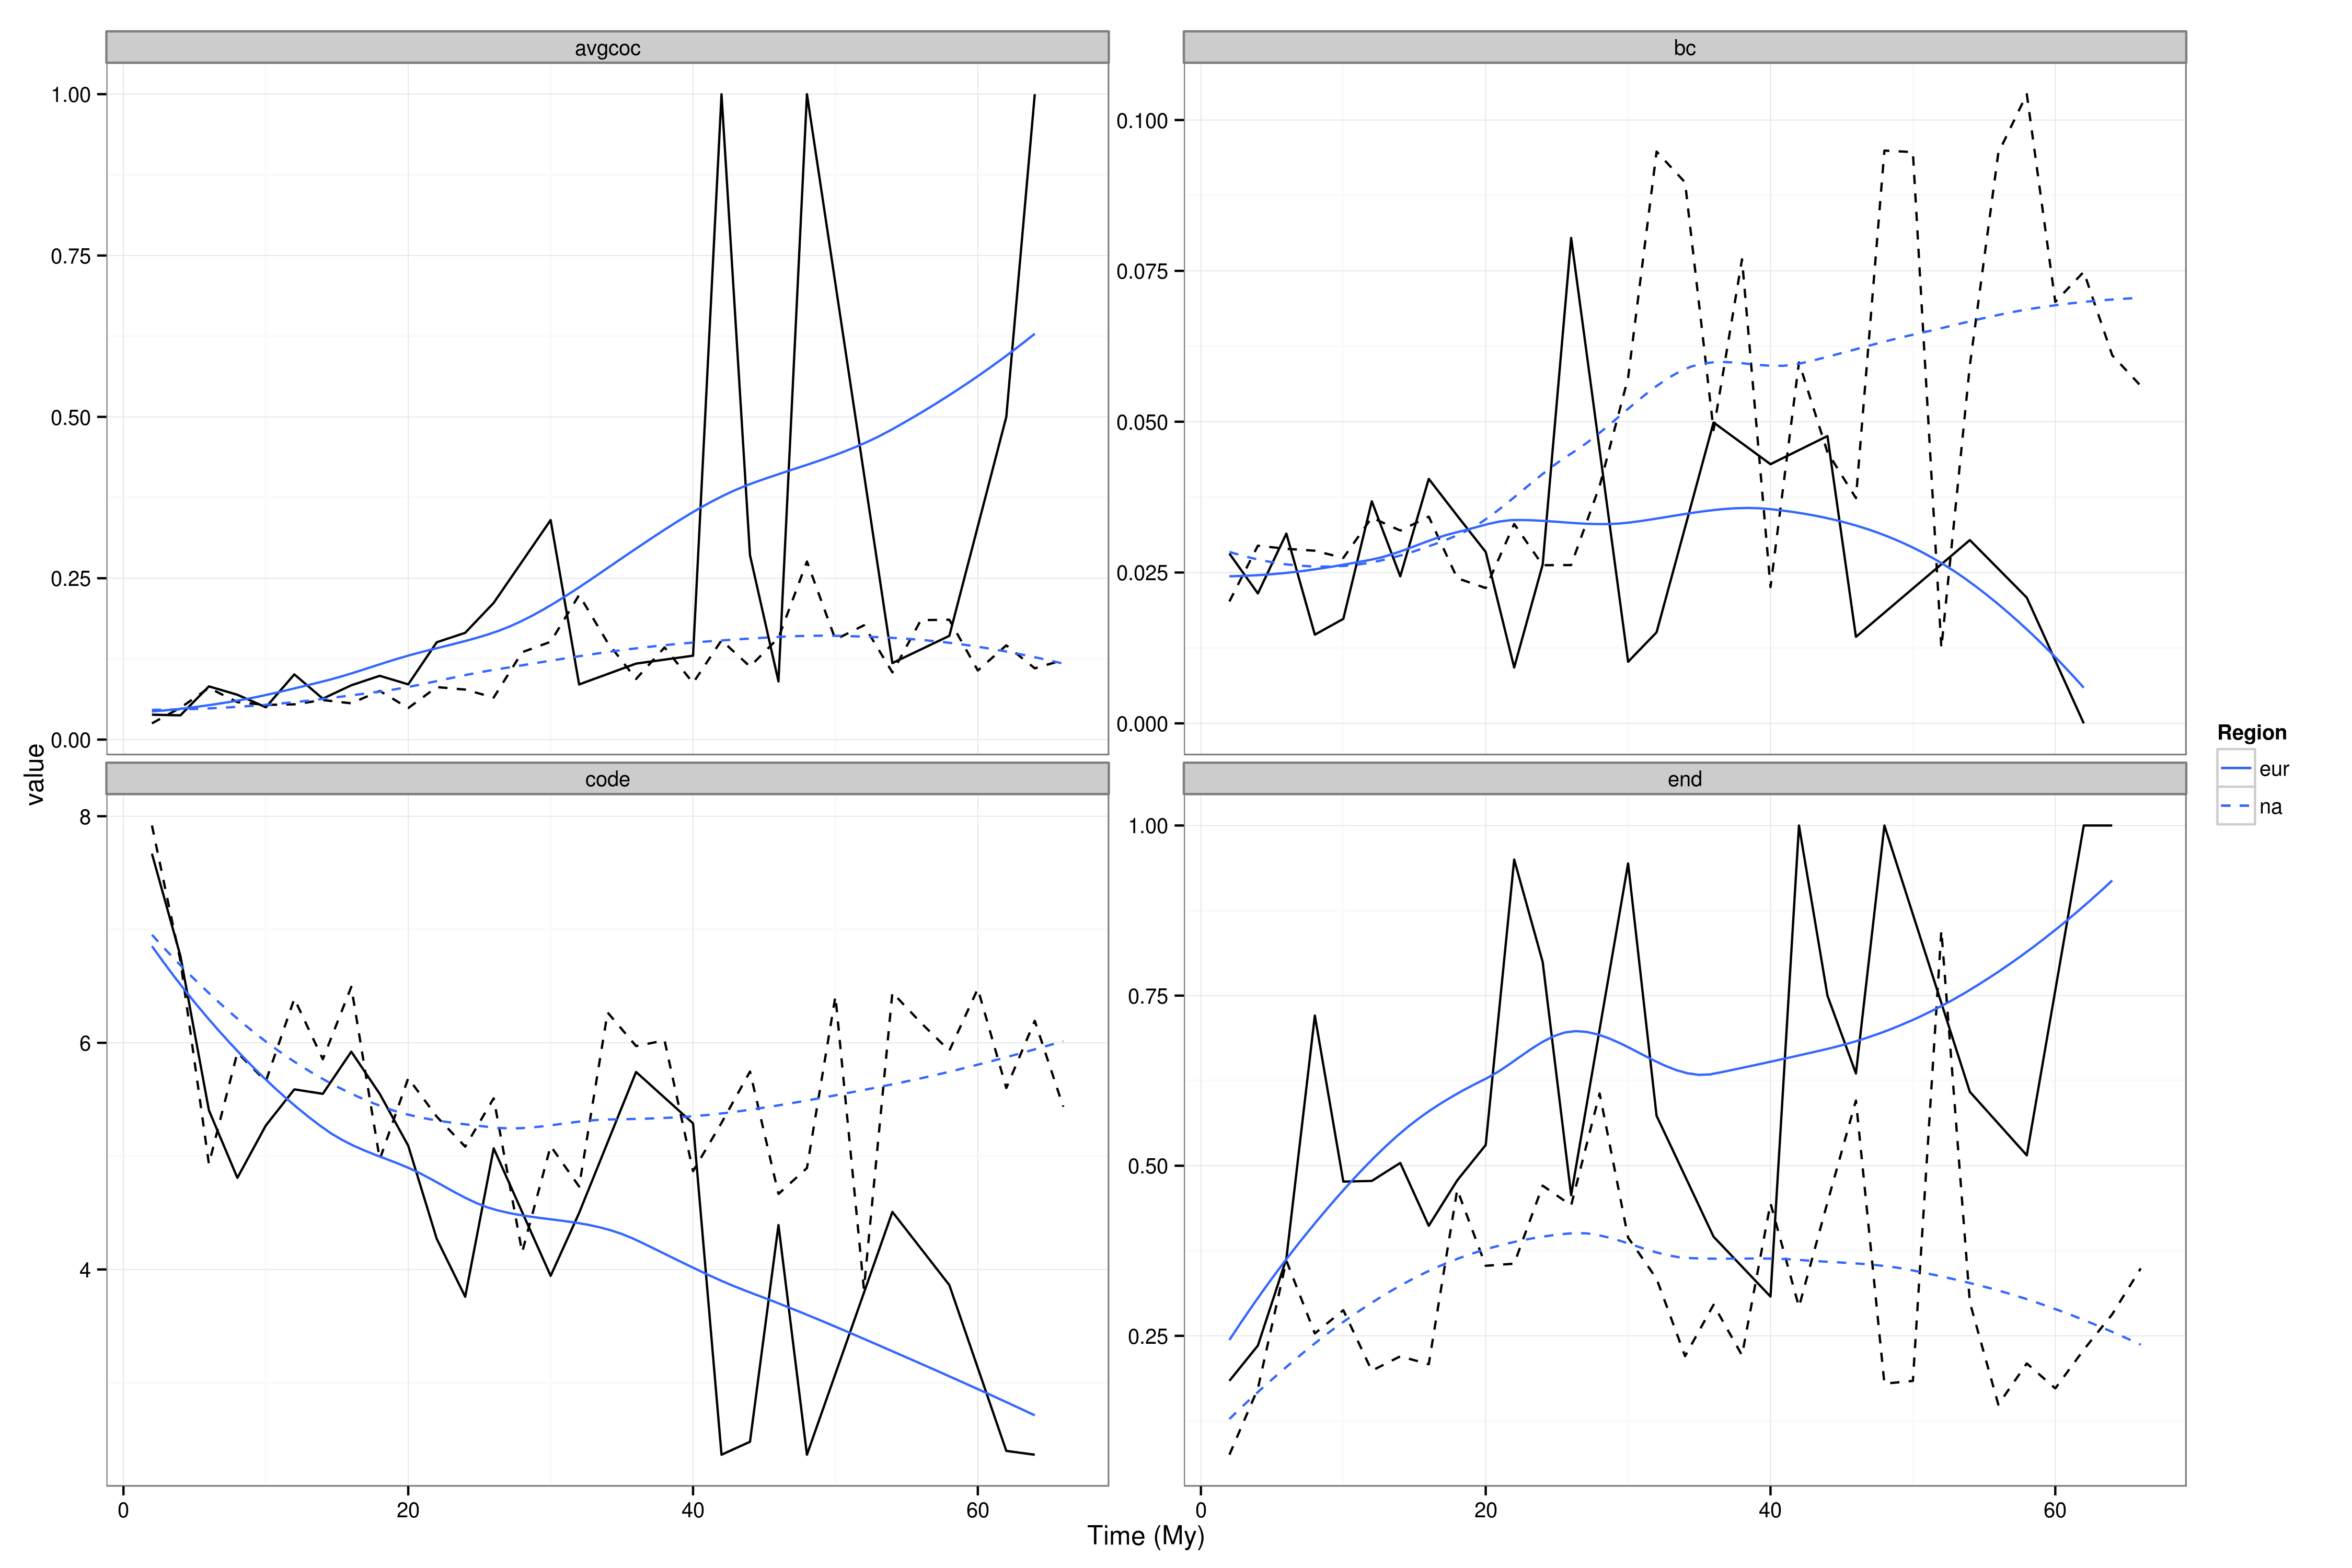
\includegraphics[height = 0.4\textheight, keepaspectratio = true]{figure/gen_bin}
  \end{center}
  \caption{Biogeographic network summary statistics for mammalian communities in North America (dashed line) and Europe (solid line). The summary statistics are, clockwise from top left: biogeographic connectedness (BC), code length, average relative locality occupancy per taxon (Occ), and average relative number of endemic taxa per locality (E). Blue lines are generalized additive model smooths and are presented to illustrate the overall pattern for each region.} 
  \label{fig:mam_tot}
\end{figure}

There is a qualitative decrease in \(Occ\) in Europe until approximately the start of the Neogene (approximately 23 My), indicating that the average taxon is becoming generally less cosmopolitan over time. In contrast, North American \(Occ\) is qualitatively stationary over the entire Cenozoic and almost always lower than that observed for Europe. This means that, on average, North American taxa are present in very few localities at any given point in time.

In Europe there is a qualitative rise in \(BC\) in the first few million years of the Cenozoic, but afterwards remains relatively stationary meaning that the average proportion of shared taxa remained qualitatively stationary. In comparison, North American \(BC\) remains stationary with a greater amount of shared taxa than Europe for the first half of the Cenozoic followed by a decrease and another plateau at the end of the Cenozoic.

In Europe, there is a over all qualitative decrease in \(E\) while in North America there is a qualitatively constant \(E\) over the Cenozoic with a slight decrease in the Neogene. As discussed above, \(E\) is a measure of relative uniqueness of a locality on average. Qualitatively, North America retained approximately the same amount of site uniqueness through out the Cenozoic. While the pattern of the European record shows a qualitatively nonmonotonic decrease in locality uniqueness.

The code length of European biogeographic networks increases qualitatively over the entire Cenozoic, while code length of North American networks remains relatively constant until the Neogene when there is a qualitative increase. Initial interpretation of these results indicates that North America maintains a relatively stationary degree of provinciality while Europe has a qualitatively decreasing degree of provinciality. 


\section{Synthesis of proposed research} \label{sec:synth}
Underlying all of the above is a foundational question in paleobiology: why do certain taxa go extinct while others do not? In the context of evolutionary paleoecology, this question can be rephrased as ``how do the set of all biotic--biotic and biotic--abiotic interactions a taxon experiences over time (i.e. adaptive zone \citealp{Simpson1944}) affect extinction risk?'' Related to this is the Law of Constant Extinction which states that extinction risk for a given adaptive zone is taxon--age independent \citep{VanValen1973}. It is asserted that the Law of Constant Extinction only holds during periods of relatively constant environment even though this was not the context for the initial observation \citep{Liow2007b,VanValen1973} which can be interpreted as the set of dominant non-organism mediated processes do not fluctuate or fluctuate in a known manner. By understanding which non-organism mediated processes may be shaping the environment (set of all possible biotic and abiotic interactors) and how they change over time and phrasing analysis of extinction in this context, it may be possible to ``test'' the Law of Constant Extinction.

The first two studies proposed above investigate how organismal traits potentially related to environmental preference affect extinction rate. In effect, these traits may determine the ``bounds'' of a taxon's adaptive zone by limiting the total set of interactions to just those for which the taxon is adapted. The final proposed study aims to estimate what non-organism mediated processes (global, regional, and/or local) may be dominate in shaping the environment and the related set of adaptive zones. Between these studies, as well the use of two desperate groups, it should be possible to determine when, what, and if certain variables matter for survival and potentially how they matter. 



\clearpage
\section{Timeline}

Spring/Summer 2014
\begin{itemize}
  \item Evolution Meeting: preliminary brachiopod survival results
  \item South American fossil mammal data from Field Museum of Natural History collections
\end{itemize}

Fall 2014/Winter 2015
\begin{itemize}
  \item GSA: survivorship simulation for anagenesis and sampling
  \item Doctoral Dissertation Improvement Grant
\end{itemize}

Spring/Summer 2015
\begin{itemize}
  \item Evolution Meeting: mammalian survivorship analysis for North America and Europe
  \item South American fossil mammal data from American Museum of Natural History collections
  \item write and submit survivorship simulation paper
\end{itemize}

Fall 2015/Winter 2016
\begin{itemize}
  \item SVP or GSA: mammalian biogeographic connectedness
  \item write and submit mammal connectedness paper
\end{itemize}

Spring/Summer 2016
\begin{itemize}
  \item Evolution Meeting: brachiopod survival analysis results
  \item write and submit brachiopod survival paper
\end{itemize}

Fall 2016/Winter 2017
\begin{itemize}
  \item SVP or GSA: mammalian survivorship analysis
  \item write and submit mammal survival paper
\end{itemize}

Spring/Summer 2017
\begin{itemize}
  \item Evolution Meeting
  \item write and submit review/philosophy paper
  \item \textbf{Defend}
\end{itemize}



\clearpage
\bibliographystyle{abbrvnat}
\bibliography{proposal}

\end{document}
